\documentclass{tufte-handout} % A4 paper and 11pt font size
\usepackage[activate={true,nocompatibility},final,tracking=true,kerning=true,spacing=true,factor=1100,stretch=10,shrink=10]{microtype}
\usepackage[T1]{fontenc} % Use 8-bit encoding that has 256 glyphs
%\usepackage{mathpazo} % Use the Adobe Utopia font for the document - comment this line to return to the LaTeX default
\usepackage[english, serbianc]{babel} % English language/hyphenation
\usepackage{amsmath,amsfonts,amsthm, amssymb} % Math packages
\usepackage{pgf,tikz}
\usetikzlibrary{positioning,matrix,arrows}
\usepackage{float}
\usepackage{tikz-cd}
\usepackage{caption}
\usepackage{stmaryrd}
\usepackage{multicol}
\usepackage{booktabs}
\usepackage{verbatim}
\usepackage{lipsum} % Used for inserting dummy 'Lorem ipsum' text into the template
\usepackage{sectsty} % Allows customizing section commands
\usepackage{titlesec}
\usepackage{empheq}
\usepackage[most]{tcolorbox}
%Boxed eqns
\newcommand{\boxedeq}[1]{\begin{empheq}[box={\fboxsep=6pt\fbox}]{align} #1\end{empheq}}

\allsectionsfont{\normalfont \bfseries} % Make all sections centered, the default font and small caps
\usepackage{enumerate}
\usepackage{pythonhighlight}
\usepackage{fancyhdr} % Custom headers and footers
\pagestyle{fancyplain} % Makes all pages in the document conform to the custom headers and footers
\fancyhead{} % No page header - if you want one, create it in the same way as the footers below
\fancyfoot[L]{} % Empty left footer
\fancyfoot[C]{} % Empty center footer
\fancyfoot[R]{\thepage} % Page numbering for right footer
\renewcommand{\headrulewidth}{0pt} % Remove header underlines
\renewcommand{\footrulewidth}{0pt} % Remove footer underlines
\setlength{\headheight}{13.6pt} % Customize the height of the header
\allowdisplaybreaks

\usepackage{wrapfig}
\graphicspath{ {./slike/} }

%Sections

%--------Theorem Environments--------
%theoremstyle{plain} --- default
\newtheorem{thm}{Theorem}
\newtheorem{cor}[thm]{Corollary}
\newtheorem{prop}[thm]{Proposition}
\newtheorem{facts}[thm]{Facts}
\newtheorem{fact}[thm]{Fact}
\newtheorem{clm}[thm]{Claim}
\newtheorem{lem}[thm]{Lemma}
\newtheorem{conj}[thm]{Conjecture}
\newtheorem{quest}[thm]{Question}

\theoremstyle{definition}
\newtheorem{defn}[thm]{Definition}
\newtheorem{defns}[thm]{Definitions}
\newtheorem{con}[thm]{Construction}
\newtheorem{exmp}[thm]{Example}
\newtheorem{exmps}[thm]{Examples}
\newtheorem{notn}[thm]{Notation}
\newtheorem{notns}[thm]{Notations}
\newtheorem{addm}[thm]{Addendum}
\newtheorem{exer}[thm]{Exercise}

\theoremstyle{remark}
\newtheorem{rem}[thm]{Remark}
\newtheorem{rems}[thm]{Remarks}
\newtheorem{warn}[thm]{Warning}
\newtheorem{sch}[thm]{Scholium}

\newcommand{\bra}[1]{\left(#1\right)}
\newcommand{\sbra}[1]{\left[#1\right]}
\newcommand{\Mod}[1]{\ (\text{mod}\ #1)}
\newcommand{\op}[1]{#1^{\text{op}}}
\newcommand{\R}{\mathbb{R}}
\newcommand{\N}{\mathbb{N}}
\newcommand{\Z}{\mathbb{Z}}
\newcommand{\mZ}{\mathcal{Z}}
\renewcommand{\C}{\mathbb{C}}
\newcommand{\Q}{\mathbb{Q}}
\newcommand{\F}{\mathbb{F}}
\newcommand{\bA}{\mathbb{A}}
\newcommand{\bH}{\mathbb{H}}
\newcommand{\one}{\mathbb{1}}
\newcommand{\mC}{\mathcal{C}}
\newcommand{\mO}{\mathcal{O}}
\newcommand{\mR}{\mathcal{R}}
\newcommand{\mS}{\mathcal{S}}
\newcommand{\lp}{{\mathfrak{p}}}
\renewcommand{\P}{\mathbb{P}}
\newcommand{\E}{\mathbb{E}}
\DeclareMathOperator{\dist}{dist}
\DeclareMathOperator{\aut}{Aut}
\DeclareMathOperator{\gal}{Gal}
\DeclareMathOperator{\var}{\textbf{var}}
\DeclareMathOperator{\orb}{Orb}
\DeclareMathOperator{\ff}{Frac}
\DeclareMathOperator{\stab}{Stab}
\DeclareMathOperator{\inn}{Inn}
\DeclareMathOperator{\Ind}{Ind}
\DeclareMathOperator{\Res}{Res}
\DeclareMathOperator{\spn}{Span}
\DeclareMathOperator{\out}{Out}
\DeclareMathOperator{\im}{Im}
\DeclareMathOperator{\rk}{rk}
\DeclareMathOperator{\disc}{disc}
\DeclareMathOperator{\tors}{Tors}
\DeclareMathOperator{\Mor}{Mor}
\DeclareMathOperator{\End}{End}
\DeclareMathOperator{\Hom}{Hom}
\DeclareMathOperator{\Nat}{Nat}
\DeclareMathOperator{\spec}{Spec}
\DeclareMathOperator{\ann}{Ann}
\DeclareMathOperator{\ord}{ord}
\DeclareMathOperator{\conjc}{Conj}
\DeclareMathOperator{\Br}{Br}
\DeclareMathOperator{\Tr}{Tr}
\DeclareMathOperator{\Nm}{Nm}
\DeclareMathOperator{\Char}{char}
\newcommand{\norm}[1]{\left\lVert #1 \right\rVert}
\newcommand{\inp}[2]{\left\langle #1, #2 \right\rangle}
\newcommand{\shreq}[2]{-\frac{\hbar^2}{2m}\frac{\partial^2 #1}{\partial #2^2} + U(#2) #1 =E #1}
\newcommand{\tshreq}[2]{i\hbar\frac{\partial #1}{\partial t^2} = -\frac{\hbar^2}{2m}\frac{\partial^2 #1}{\partial #2^2} + U(#2) #1}
\newcommand{\kpsi}{\psi^{''}+k\psi=0}
\def \v {\vspace{0.2cm}}

\geometry{
	left=13mm, % left margin
	textwidth=130mm, % main text block
	marginparsep=8mm, % gutter between main text block and margin notes
	marginparwidth=55mm % width of margin notes
}
\fontsize{10}{20}\selectfont
%----------------------------------------------------------------------------------------
%	TITLE SECTION
%----------------------------------------------------------------------------------------

\title{	
	\normalfont\normalsize 
	{Електротехнички факултет, Универзитет у Београду - Летњи семестар 2023.} \\ [0pt] % Your university, school and/or department name(s)
	\huge Белешке - Квантна Механика% The assignment title
}\author{Михаило Стојковић} % Your name
\date{\vspace{-5pt}\normalsize\today} % Today's date or a custom date


\titleformat{\section}
	{}{\noindent\rule{\textwidth}{0.5pt}\\thesection\\\noindent\rule{\textwidth}{0.5pt} }{1em}{}[{\titlerule[0.8pt]}]




\begin{document}
\justifying 
\maketitle

\tableofcontents


\section{Предавање - 8.3.2023.}
Само предавање креће са тим да посматрамо стационарну Шредингерову једначину:
	\boxedeq{\shreq{\psi}{x}}
али у случају када је $U(x)=0$. Заменом $k^2\equiv\frac{2mE}{\hbar^2}$ у претходну једначину\footnote{Оваква смена се често појављује у курсу тако да после неког времена постане стандардно да када год се појави неко $k$ сматрамо да је једнако наведеном изразу} добијамо диференцијалну једначину:
	\boxedeq{\label{eqn:sred_k}\kpsi}
Решење ове диференцијалне једначине можемо изразити у два облика:
\begin{enumerate}
	\item Као збир експоненцијала\footnote{Овај облик решења је јако користан у ситуацијама где нам се Шредингерова једначина сведе на облик сличан једначини (\ref{eqn:sred_k}), где ако је испред коефицијента уз $\psi$ знак минус, функција ће бити чисто реална. Решења у овом облику се често узимају у ситуацијама где разматрамо константну потенцијалну енергију или честицу која се налази у коначној баријери}: $\psi(x)=Ae^{ikx} + Be^{-ikx}$
	\item Као збир синуса и косинуса\footnote{Овај облик решења је јако користан ако на интервалу решавања имамо неку бесконачну баријеру}: $\psi(x)=C\sin(kx)+D\cos(kx)$
\end{enumerate}
Оба облика су решење дате диференцијалне једначине и може се лако показати како једно можемо представити преко другог.\par
Посматрамо решење у експоненцијалном облику. Због хомогености диференцијалне једначине, негативно и позитивно решење можемо посматрати као два засебна решења са додатом функцијом времена.
\begin{align}
	\label{eqn:talas_u_desno}\psi_1(x,t)&=A_1e^{i(kx-\omega t)}\\
	\label{eqn:talas_u_levo}\psi_2(x,t)&=B_1e^{-i(kx-\omega t)} 
\end{align}
и заправо, једначина (\ref{eqn:talas_u_desno}) представља талас који се креће на десно, а једначина (\ref{eqn:talas_u_levo}) представља талас који се креће на лево.

\begin{wrapfigure}{l}{0.5\textwidth}
	\centering
	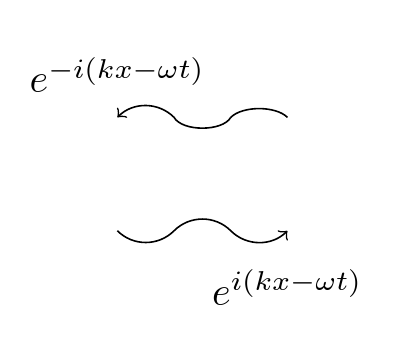
\includegraphics[width=0.5\textwidth]{kretanje_talasa.png}
	\caption{Кретање таласа}
\end{wrapfigure}
Питање које се увек поставља при добитку неког решења једначине: "Да ли ово може представљати таласну једначину". Услови који морају бити испуњени за таласну функцију на неком интервалу су следећи:
\begin{enumerate}
	\item Таласна функција мора бити нормирана
	\item Таласна функција мора бити непрекидна
	\item Први извод таласна функције мора бити непрекидан
\end{enumerate}
При почетку решавања проблема нисмо експлицитно специфицирали интервал решавања, тако да сматрамо да је интервал цело поље $\R$. Овде настаје сада проблем јер решење које смо добили не може да се нормира.
\begin{align}
	\int_{-\infty}^{+\infty}\psi_1^{\ast}\psi_1 dx = |A_1|^2\int_{-\infty}^{+\infty}dx\nless \infty\\ 
	\int_{-\infty}^{+\infty}\psi_2^{\ast}\psi_2 dx = |B_1|^2\int_{-\infty}^{+\infty}dx\nless \infty\\
\end{align}
\section{Предавање - 10.3.2023.}
\section{Предавање - 22.3.2023.}
\section{Предавање - 24.3.2023.}
\section{Предавање - 29.3.2023.}
\section{Предавање - 5.4.2023.}
\section{Предавање - 7.4.2023.}
\section{Предавање - 12.4.2023.}








\end{document}